\section{Моделі та алгоритми для управління розподільчими логістичними системами}
\subsection{Опис агентів системи}
Схема агентів та використовуваємих їми моделей системи представлена на рисунку~\ref{fig:agent_scheme}.

\begin{figure}[H]
	\centering
	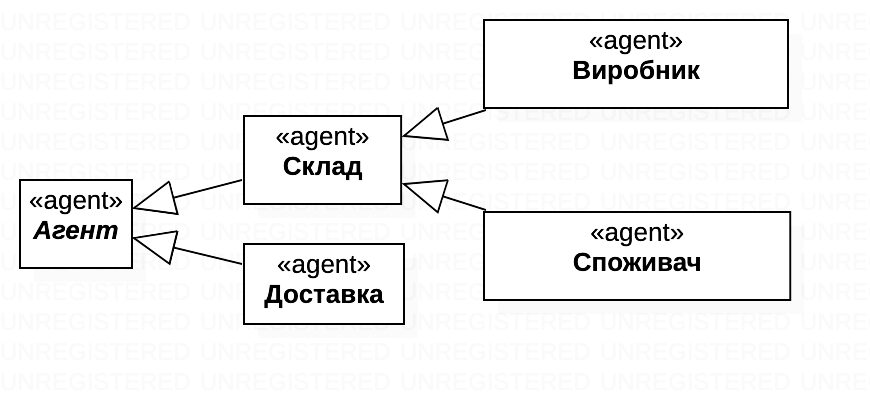
\includegraphics[width=\textwidth]{agent_scheme}
	\caption{Схема агентів та моделей системи}
	\label{fig:agent_scheme}
\end{figure} 

Цілями кінцевих агентів системи є:

\begin{enumerate}
	\item Попит --- симуляція реального попиту на товари.
	\item Склад:
	\begin{enumerate}[label={2.\arabic*}]
		\item Зменшити вартість зберігання запасу, замовляючи ретельно розраховану кількість товарів;
		\item Доставка товарів без затримок.
	\end{enumerate}
	\item Роздрібний торговець:
	\begin{enumerate}[label={3.\arabic*}]
		\item Зменшити вартість зберігання запасу, замовляючи ретельно розраховану кількість товарів згідно до прогнозу попиту;
		\item Коли рівень запасу знижується до критичного, то роздрібний торговець повинен надіслати замовлення до найближчих інших точок, щоб екстрено збільшити рівень запасу;
		\item Коли рівень запасу занадто великий, то він може надіслати частину товару до інших точок.
	\end{enumerate}
\end{enumerate}

\subsection{Опис моделей агентів системи}
\subsubsection{Розрахунок витрат на запаси}
Загальні витрати, пов'язані з запасами, представляють собою суму витрат на закупівлю, поповнення запасу і утримання запасів~\cite{Sterligova2008}:
\begin{equation} \label{eq:t}
T=C\cdot S+\cfrac{S}{C}\cdot A+(Z_s+\cfrac{Q}{2}\cdot I)
,
\end{equation}
\begin{description}
	\item[де] $T$ --- загальні витрати, пов'язані з запасом, г.~о.;
	\item $C$ --- закупівельні ціна одиниці товару, г.~о.;
	\item $Q$ --- розмір замовлення, одиниць;
	\item $S$ --- обсяг потреби в запасі, одиниць;
	\item $A$ --- витрати на виконання одного замовлення, г.~о.;
	\item $Z_s$ --- розмір страхового запасу, одиниць;
	\item $I$ --- витрати на утримання одиниці запасу, г.~о.
\end{description}

\subsubsection{Розрахунок оптимального розміру поповнення запасу}
В основі оптимізації рівня запасу лежить розрахунок розміру замовлення, який може забезпечити оптимальний рівень запасу при обслуговуванні на заданому рівні.
Критерієм оптимізації при цьому є, як правило, мінімум загальних витрат, пов'язаних з запасами.

Формула Вільсона --- найбільш відомий і широко вживаний метод розрахунку розміру замовлення~\cite{Sterligova2008}:
\begin{equation}
Q^*=\cfrac{dT}{dQ}=\sqrt{\cfrac{2\cdot A\cdot S}{I}}
,
\end{equation}
\begin{description}
	\item[де] $T$ --- загальні витрати~\eqref{eq:t}, пов'язані з запасом, г.~о.;
	\item $Q$ --- розмір замовлення, одиниць;
	\item $S$ --- обсяг потреби в запасі, одиниць;
	\item $A$ --- витрати на виконання одного замовлення, г.~о.;
	\item $I$ --- витрати на утримання одиниці запасу, г.~о.;
	\item $Q^*$ --- оптимальний розмір замовлення, одиниць.
\end{description}

\subsubsection{Моделі управління запасами}
\paragraph{Модель з фіксованим розміром замовлень}
Методика управління запасами на основі фіксації розміру замовлення~(рисунок~\ref{fig:model_fs:dynamic}) полягає в тому, що замовлення на поповнення запасу робляться в момент зниження запасу до визначеного порогового рівня запасу, що дорівнює оптимальному розміру замовлення~\cite{Sterligova2008}. 

\begin{figure}[H]
  \centering
\begin{tikzpicture}
  \begin{axis}[ 
    xlabel={Час},
    ylabel={Запас},
    xmin=0,xmax=10,ymin=0,ymax=1
  ] 
	\addplot
		coordinates {
			(0,0.8) [0]
			(3,0.2) [1]
			(3,0.9) [2]
			(7,0.25) [3]
			(7,0.95) [4]
			(9,0.1) [5]
			(9,0.8) [6]
			(10,0.5) [7]
		};
	\draw[<->] (axis cs:2.8,0.2) -- node[left]{\footnotesize $Q$} (axis cs:2.8,0.9);

    \draw [densely dotted] (axis cs:0,0.4) -- node[below]{\footnotesize Пороговий запас} (axis cs:10,0.4);
    \draw [densely dotted] (axis cs:0,0.2) -- node[below]{\footnotesize Страховий запас} (axis cs:10,0.2);
  \end{axis}
\end{tikzpicture}
  \captionsetup{justification=centering}
  \caption{Динаміка запасу в моделі управління з фіксованим розміром замовлень}
  \label{fig:model_fs:dynamic}
\end{figure}

Максимальний бажаний запас може бути розрахований таким чином~\cite{Sterligova2008}:
\begin{equation} \label{eq:model_fs:mws}
MWS=Q^*+Z_s
,
\end{equation}
\begin{description}
	\item[де] $MWS$ --- максимальний бажаний запас, одиниць;
	\item $Q^*$ --- оптимальний розмір замовлення;
	\item $Z_s$ --- обсяг страхового запасу, одиниць.
\end{description}

Розмір страхового запасу може бути розрахований різними методами.
Метод прямого рахунку~\cite{Sterligova2008}:
\begin{equation} \label{eq:model_fs:zs1}
Z_s=C_d-t_{od}
,
\end{equation}
\begin{description}
	\item[де] $C_d$ --- очікуване денне споживання, одиниць;
	\item $t_{od}$ --- час затримки постачання, дні.
\end{description}

Страховий запас визначається як різниця між максимальним споживанням під час виконання замовлення і очікуваним споживання під час виконання замовлення~\cite{Sterligova2008}:
\begin{equation} \label{eq:model_fs:zs2}
Z_s=MC-EC
,
\end{equation}
\begin{description}
	\item[де] $MC$ --- максимальне споживання за час виконання замовлення, одиниць;
	\item $EC$ --- очікуване споживання за час виконання замовлення, одиниць.
\end{description}

У свою чергу максимальне споживання за час виконання замовлення розраховується по формулі~\cite{Sterligova2008}:
\begin{equation}
MC=C_d\cdot(t_d+t_{od})
,
\end{equation}
\begin{description}
	\item[де] $t_d$ --- час виконання замовлення, дні.
\end{description}

Очікуване денне споживання $C_d$ розраховується виходячи з очікуваної потреби в запасі за весь період~\cite{Sterligova2008}:
\begin{equation}
S_d=\cfrac{S}{N}
,
\end{equation}
\begin{description}
	\item[де] $S_d$ --- очікуване денне споживання, одиниць;
	\item $S$ --- обсяг потреби в запасі, одиниць;
	\item $N$ --- число робочих днів у плановому періоді.
\end{description}

Очікуване споживання за час виконання замовлення $EC$ розраховується як добуток очікуваного денного споживання на час виконання замовлення~\cite{Sterligova2008}:
\begin{equation}
EC=S_d\cdot t_d
,
\end{equation}
\begin{description}
	\item[де] $EC$ --- очікуване споживання за час виконання замовлення, одиниць.
\end{description}

Страхових запас $Z_s$ може також бути розрахований за іншими формулами, які мають статистичний, імовірнісний або емпіричній характер~\cite{Sterligova2008}.

\paragraph{Модель з фіксованим інтервалом часу між замовленнями}
У моделі з фіксованим інтервалом часу між замовленнями  \textit{(fixed order interval model)} замовлення робляться в строго певні моменти часу, які знаходяться один від одного на рівні інтервали (рисунок~\ref{fig:model_fi:dynamic}).

\begin{figure}[H]
  \centering
\begin{tikzpicture}
  \begin{axis}[ 
    xlabel={Час},
    ylabel={Запас},
    xmin=0,xmax=10,ymin=0,ymax=1
  ] 
	\addplot
		coordinates {
			(0,0.8) [0]
			(3,0.2) [1]
			(3,0.8) [2]
			(7,0.25) [3]
			(7,0.9) [4]
			(9,0.1) [5]
			(9,0.8) [6]
			(10,0.5) [7]
		};
	\draw[<->] (axis cs:2.8,0.2) -- node[left]{\footnotesize $Q_i$} (axis cs:2.8,0.8);
   
    \draw [dashed] (axis cs:1.5,0) -- node[left]{\footnotesize Зам.} (axis cs:1.5,1);
    \draw [dashed] (axis cs:4.5,0) -- node[left]{\footnotesize Зам.} (axis cs:4.5,1);
    \draw [dashed] (axis cs:7.5,0) -- node[left]{\footnotesize Замовлення} (axis cs:7.5,1);

    \draw [densely dotted] (axis cs:0,0.4) -- node[below]{\footnotesize Пороговий запас} (axis cs:10,0.4);
    \draw [densely dotted] (axis cs:0,0.2) -- node[below]{\footnotesize Страховий запас} (axis cs:10,0.2);
  \end{axis}
\end{tikzpicture}
  \captionsetup{justification=centering}
  \caption{Динаміка запасу в моделі з фіксованим інтервалом часу між замовленнями}
  \label{fig:model_fi:dynamic}
\end{figure}

Фіксований інтервал часу між замовленнями повинен мати оптимальний розмір. 
Оптимізація рівня запасу зв'язується з оптимізацією розміру замовлення на заповнення запасу. 
Таким чином, визначати оптимальний інтервал часу між замовленнями слід на основі оптимального розміру замовлення. 
Оптимальний розмір замовлення дозволяє мінімізувати сукупні витрати на утримання та поповнення запасу, а також досягти найкращого поєднання таких факторів, як використовувана площа складських приміщень, витрати на зберігання запасу і вартість замовлення~\cite{Sterligova2008}.

Формула для розрахунку інтервалу між замовленнями~\cite{Sterligova2008}:
\begin{equation} \label{eq:model_fi:time}
t_d=\cfrac{N\cdot Q^*}{S}
,
\end{equation}
\begin{description}
	\item[де] $t_d$ --- інтервал часу між замовленнями, дні;
	\item $N$ --- число робочих днів у плановому періоді, дні;
	\item $Q^*$ --- оптимальний розмір замовлення;
	\item $S$ --- обсяг потреби в запасі, одиниць.
\end{description}

Отриманий за допомогою формули~\eqref{eq:model_fi:time} інтервал часу між замовленнями не є обов'язковим.
Він може бути скоригований на основі експертних оцінок.

Максимальний бажаний запас визначається для відстеження доцільності завантаження площ складу з точки зору критерію мінімізації сукупних логістичних витрат.

Максимальний бажаний запас, як видно з рисунку~\ref{fig:model_fi:dynamic}, може бути розрахований таким чином~\cite{Sterligova2008}:
\begin{equation} \label{eq:model_fi:mws}
MWS=EC_t+Z_s
,
\end{equation}
\begin{description}
	\item[де] $MWS$ --- максимальний бажаний запас, одиниць;
	\item $EC_t$ --- очікуване споживання за інтервал часу між замовленнями;
	\item $Z_s$ --- обсяг страхового запасу, одиниць.
\end{description}

З урахуванням формули~\eqref{eq:model_fi:mws} розмір замовлення може бути розрахований за формулами~\cite{Sterligova2008}:
\begin{equation} \label{eq:order}
Q_i=EC_t+Z_s-Z_{Ti}-Z_t
,
\end{equation}
\begin{equation} \label{eq:order2}
Q_i=MWS-Z_{Ti}+EC-Z_{ti}
,
\end{equation}
\begin{description}
	\item[де] $Q_i$ --- розмір замовлення $i$, одиниць;
	\item $EC$ --- очікуване споживання за час виконання замовлення, одиниць;
	\item $Z_t$ --- обсяг запасу у дорозі, одиниць.
	\item $Z_{ti}$ --- обсяг запасу у дорозі, не отриманого до моменту видачі замовлення $i$, одиниць;
	\item $Z_{Ti}$ --- обсяг поточного запасу при видачі замовлення $i$, одиниць;
\end{description}

Страховий запас (формули~\ref{eq:model_fs:zs1},~\ref{eq:model_fs:zs2}) дозволяє задовольняти потребу в запасі на час передбачуваної затримки постачання.
При цьому під можливою затримкою постачання мається на увазі максимальна можлива затримка.

\paragraph{Порівняння основних моделей управління запасами}
Слід зазначити, що основні моделі управління запасами можуть застосовуватися лише до досить обмеженого спектру умов функціонування і взаємодії постачальників і споживачів.

Модель з фіксованим розміром замовлення вимагає безперервного обліку поточного запасу на складі.
Це призводить до підвищення витрат її використання.
Однак максимальний бажаний запас в цій моделі, як правило, має менший розмір, ніж в моделі з фіксованим інтервалом часу між замовленнями в зв'язку з прив'язкою інтервалу часу між замовленнями до календаря.

В цілому можна відзначити, що модель з фіксованим розміром замовлення в порівнянні з моделлю з фіксованим інтервалом часу між замовленнями частіше призводить до економії витрат на утримання запасів на складі за рахунок скорочення площ під запасами.
У той же час модель з фіксованим інтервалом часу між замовленнями вимагає лише періодичного контролю кількості запасів.
Це спрощує процедуру використання моделі і скорочує операційні витрати.

\subsubsection{Розрахунок рівня сервісу}
Розрахунок рівня логістичного обслуговування відбувається за наступною формулою~\cite{Sterligova2008}:
\begin{equation}
Y=\cfrac{m}{M} \cdot 100\%
,
\end{equation}
\begin{description}
	\item[де] $Y$ --- рівень логістичного обслуговування;
	\item $m$ --- кількісна оцінка фактичного обсягу логістичних послуг;
	\item $M$ --- кількісна оцінка теоретично можливого обсягу логістичного сервісу.
\end{description}

\subsubsection{Прогнозування числових рядів}
\textit{Порівяння та вибір моделі прогнозування числових рядів.}

\subsubsection{Модель динаміки попиту}
\textit{Порівяння та вибір моделі динаміки попиту.}

% \subsection{Метрики для оцінки моделі}
% У якості метрики для оцінкі розробленої моделі було вибрано стандартне відхилення від рівня сервису існуючої системи:
% \begin{equation}
% E = \sqrt{\frac{1}{2} \cdot \left(Y_{model} - Y_{real} \right)^2}
% ,
% \end{equation}
% \begin{description}
% 	\item[де] $Y_{model}$ --- змодельований рівень сервісу;
% 	\item $Y_{real}$ --- реальний рівень сервісу змодельованої логістичної системи.  
% \end{description}



